\section{Experimemts}
\label{sec:experiments}

We realize extensive experiments, changing the number of clusters ($K$), changing the minimum size of each component ($threshold$) and different combinations of features. In order to measure each hiperparmeter setup we consider mean Average Precision (mAP)\footnote{\url{https://en.wikipedia.org/wiki/Information_retrieval\#Mean_average_precision}} and mean Reciprocal Rank\footnote{\url{https://en.wikipedia.org/wiki/Mean_reciprocal_rank}}, both metrics are widely used in image retrieval. 

mAP considers the numbert of thruth-ground elements retrieved between the first $k$ responses, a value of 1 indicates that the whole first $k$ retrieved elements belong to the desired class, while 0 is its worst value. Mean Reciprocal Rank considers the first position of a relevant result. In the case of mAP we evaluate over the first 5 responses.

The following tables show the resuls for different hiperparameters setups, the header of each table shows the values for $K$, distance metric and $threshold$. $X$ indicates the features used in the setup. Best results are in bold.

\begin{table}[H]
\centering

\begin{tabular}{|c|c|c|c|c|c|c|r|r|}
\hline
\multicolumn{2}{|l|}{\textit{\textbf{K(clusters): 4}}} & \multicolumn{2}{l|}{\textit{\textbf{Distance : l2-norm}}} & \multicolumn{3}{l|}{\textit{\textbf{Threshold : 100}}} & \multicolumn{2}{l|}{\textit{\textbf{K(metric MAP) :  5}}} \\ \hline
\multicolumn{7}{|c|}{\textbf{Features}} & \multicolumn{2}{c|}{\textbf{Metrics}} \\ \hline
\textbf{Region Size} & \textbf{Mean Color} & \textbf{Contrast} & \textbf{Correlation} & \textbf{Entropy} & \textbf{Centroid} & \textbf{Bound Box} & \multicolumn{1}{c|}{\textbf{MRR}} & \multicolumn{1}{c|}{\textbf{MAP}} \\ \hline
X & X & X & X & X & X & X & 0.513 & 0.467 \\ \hline
- & X & X & X & X & X & X & 0.723 & 0.671 \\ \hline
X & X & X & X & X & X & - & 0.495 & 0.456 \\ \hline
- & X & X & X & X & X & - & 0.673 & 0.638 \\ \hline
\textit{\textbf{-}} & \textit{\textbf{X}} & \textit{\textbf{X}} & \textit{\textbf{X}} & \textit{\textbf{X}} & \textit{\textbf{-}} & \textit{\textbf{-}} & \textit{\textbf{0.744}} & \textit{\textbf{0.696}} \\ \hline
\end{tabular}


\caption{Results for L2-norm distance, threshold 100 for conected components and k=4 for K-means}
\label{table:results01}
\end{table}


\begin{table}[H]
\centering
\begin{tabular}{|c|c|c|c|c|c|c|r|r|}
\hline
\multicolumn{2}{|l|}{\textit{\textbf{K(clusters): 4}}} & \multicolumn{2}{l|}{\textit{\textbf{Distance : cosine}}} & \multicolumn{3}{l|}{\textit{\textbf{Threshold : 100}}} & \multicolumn{2}{l|}{\textit{\textbf{K(metric MAP) :  5}}} \\ \hline
\multicolumn{7}{|c|}{\textbf{Features}} & \multicolumn{2}{c|}{\textbf{Metrics}} \\ \hline
\textbf{Region Size} & \textbf{Mean Color} & \textbf{Contrast} & \textbf{Correlation} & \textbf{Entropy} & \textbf{Centroid} & \textbf{Bound Box} & \multicolumn{1}{c|}{\textbf{MRR}} & \multicolumn{1}{c|}{\textbf{MAP}} \\ \hline
\textit{X} & \textit{X} & \textit{X} & \textit{X} & \textit{X} & \textit{X} & \textit{X} & 0.774 & 0.738 \\ \hline
\textit{-} & \textit{X} & \textit{X} & \textit{X} & \textit{X} & \textit{X} & \textit{X} & 0.774 & 0.738 \\ \hline
\textit{X} & \textit{X} & \textit{X} & \textit{X} & \textit{X} & \textit{X} & \textit{-} & 0.774 & 0.738 \\ \hline
\textit{-} & \textit{X} & \textit{X} & \textit{X} & \textit{X} & \textit{X} & \textit{-} & 0.774 & 0.738 \\ \hline
\textit{-} & \textit{X} & \textit{X} & \textit{X} & \textit{X} & \textit{-} & \textit{-} & 0.774 & 0.738 \\ \hline
\end{tabular}
\caption{Results for Cosine distance, threshold 100 for conected components and k=4 for K-means}
\label{table:results02}
\end{table}


\begin{table}[H]
\centering
\begin{tabular}{|c|c|c|c|c|c|c|r|r|}
\hline
\multicolumn{2}{|l|}{\textit{\textbf{K(clusters): 4}}} & \multicolumn{2}{l|}{\textit{\textbf{Distance : L2-norm}}} & \multicolumn{3}{l|}{\textit{\textbf{Threshold : 300}}} & \multicolumn{2}{l|}{\textit{\textbf{K(metric MAP) :  5}}} \\ \hline
\multicolumn{7}{|c|}{\textbf{Features}} & \multicolumn{2}{c|}{\textbf{Metrics}} \\ \hline
\textbf{Region Size} & \textbf{Mean Color} & \textbf{Contrast} & \textbf{Correlation} & \textbf{Entropy} & \textbf{Centroid} & \textbf{Bound Box} & \multicolumn{1}{c|}{\textbf{MRR}} & \multicolumn{1}{c|}{\textbf{MAP}} \\ \hline
X & X & X & X & X & X & X & 0.499 & 0.456 \\ \hline
- & X & X & X & X & X & X & 0.683 & 0.637 \\ \hline
X & X & X & X & X & X & - & 0.472 & 0.437 \\ \hline
- & X & X & X & X & X & - & 0.619 & 0.545 \\ \hline
\textit{\textbf{-}} & \textit{\textbf{X}} & \textit{\textbf{X}} & \textit{\textbf{X}} & \textit{\textbf{X}} & \textit{\textbf{-}} & \textit{\textbf{-}} & \textit{\textbf{0.714}} & \textit{\textbf{0.6745}} \\ \hline
\end{tabular}
\caption{Results for L2-norm distance, threshold 300 for conected components and k=4 for K-means}
\label{table:results03}
\end{table}


\begin{table}[H]
\centering
\begin{tabular}{|c|c|c|c|c|c|c|r|r|}
\hline
\multicolumn{2}{|l|}{\textit{\textbf{K(clusters): 8}}} & \multicolumn{2}{l|}{\textit{\textbf{Distance : L2-norm}}} & \multicolumn{3}{l|}{\textit{\textbf{Threshold : 300}}} & \multicolumn{2}{l|}{\textit{\textbf{K(metric MAP) :  5}}} \\ \hline
\multicolumn{7}{|c|}{\textbf{Features}} & \multicolumn{2}{c|}{\textbf{Metrics}} \\ \hline
\textbf{Region Size} & \textbf{Mean Color} & \textbf{Contrast} & \textbf{Correlation} & \textbf{Entropy} & \textbf{Centroid} & \textbf{Bound Box} & \multicolumn{1}{c|}{\textbf{MRR}} & \multicolumn{1}{c|}{\textbf{MAP}} \\ \hline
X & X & X & X & X & X & X & 0.414 & 0.360 \\ \hline
\textit{\textbf{-}} & \textit{\textbf{X}} & \textit{\textbf{X}} & \textit{\textbf{X}} & \textit{\textbf{X}} & \textit{\textbf{X}} & \textit{\textbf{X}} & \textit{\textbf{0.786}} & \textit{\textbf{0.745}} \\ \hline
X & X & X & X & X & X & - & 0.395 & 0.341 \\ \hline
- & X & X & X & X & X & - & 0.737 & 0.685 \\ \hline
- & X & X & X & X & - & - & 0.769 & 0.734 \\ \hline
\end{tabular}
\caption{Results for L2-norm distance, threshold 300 for conected components and k=8 for K-means}
\label{table:results03}
\end{table}

Comparing tables \ref{table:results01} and \ref{table:results01} we can see that cosine distance seems to be better than L2-norm distance, but we found something particularly extrange, all the resulst for cosine distance are the same, this may be just a coinsidence but if we consider that in the rest of expiments, the use of the region of size always decrease the results it is expected this to happen also for the cosine distance.

Comparing tables \ref{table:results01} and \ref{table:results02} we can see that $threshold$ for the size of the components has an interesting effect, in general considering some small areas is good, but this has relation with the numbers of clusters considered, in the case of table \ref{table:results03} it has better results but with a greater value for $threshold$ and this is because the number of clusters considered is 8 and this creates much more components.

Based on the results, the best hiperparameter setup is \textbf{\textit{K = 8} for the number of clusters, L2-norm for the distance metric, 300 for \textit{threshold} in the conected components, and mean color, constrat, correlation, entropy, centroit and bounding box as features}, the best 3 results for  specific queries with the best hiperpameters are:

\begin{itemize}
\item \textbf{beach\_2}: crater\_3, beach\_4, crater\_5 (figure\ref{fig:results_beach_2}).

\begin{figure}[H]
	\centering
	\begin{subfigure}{0.25\textwidth}
	  \centering
	  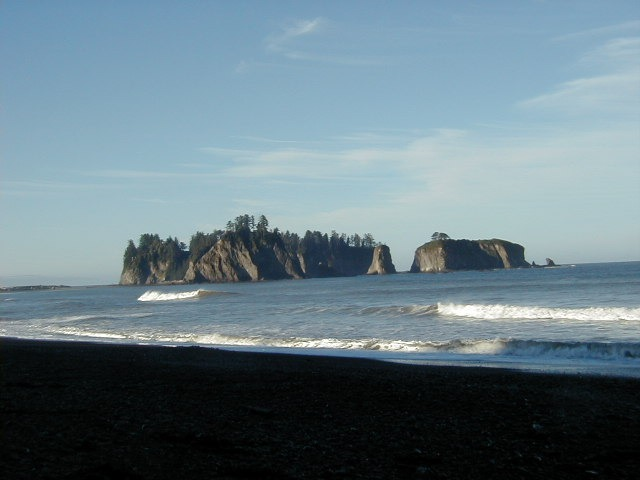
\includegraphics[width=0.9\linewidth]{../input/beach_2.jpg}
	  \caption{Query: beach\_2}
	\end{subfigure}%
	\begin{subfigure}{0.25\textwidth}
	  \centering
	  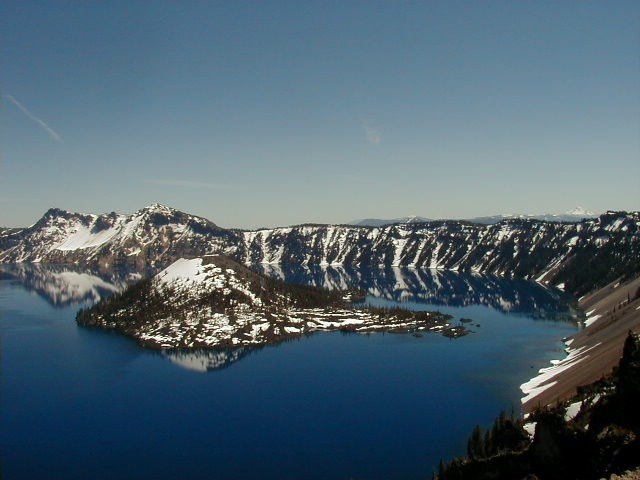
\includegraphics[width=0.9\linewidth]{../input/crater_3.jpg}
	  \caption{1st: crater\_3}
	\end{subfigure}%
	\begin{subfigure}{0.25\textwidth}
        \centering
        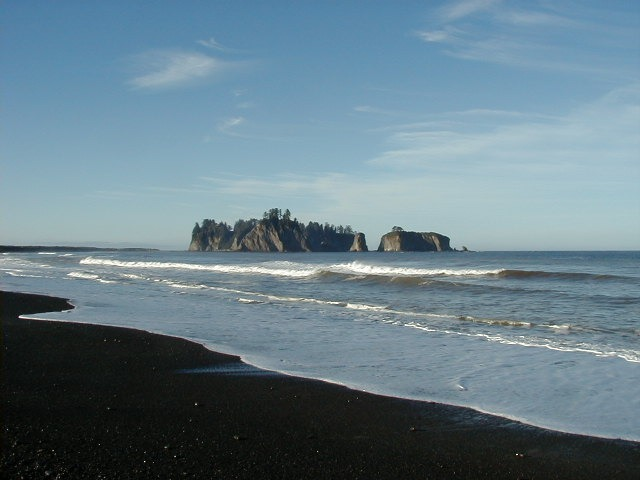
\includegraphics[width=0.9\linewidth]{../input/beach_4.jpg}
        \caption{2nd: beach\_4}
    \end{subfigure}%
    \begin{subfigure}{0.25\textwidth}
	  \centering
	  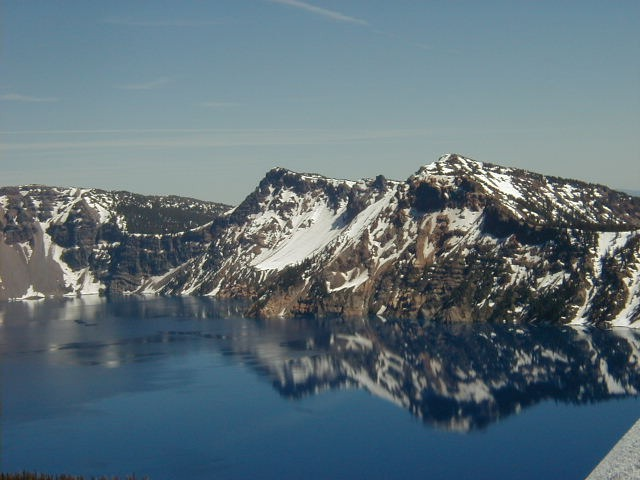
\includegraphics[width=0.9\linewidth]{../input/crater_5.jpg}
	    \caption{3th: crater\_5}
	\end{subfigure}
    \caption{Results for beach\_2}
    \label{fig:results_beach_2}
\end{figure}

\item \textbf{boat\_5}: boat\_2, cherry\_3, boat\_4 (figure \ref{fig:results_boat_5}).
\begin{figure}[H]
	\centering
	\begin{subfigure}{0.25\textwidth}
	  \centering
	  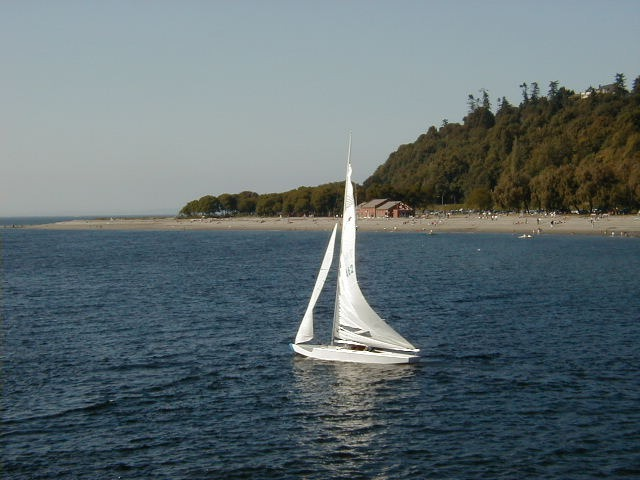
\includegraphics[width=0.9\linewidth]{../input/boat_5.jpg}
	  \caption{Query: boat\_5}
	\end{subfigure}%
	\begin{subfigure}{0.25\textwidth}
	  \centering
	  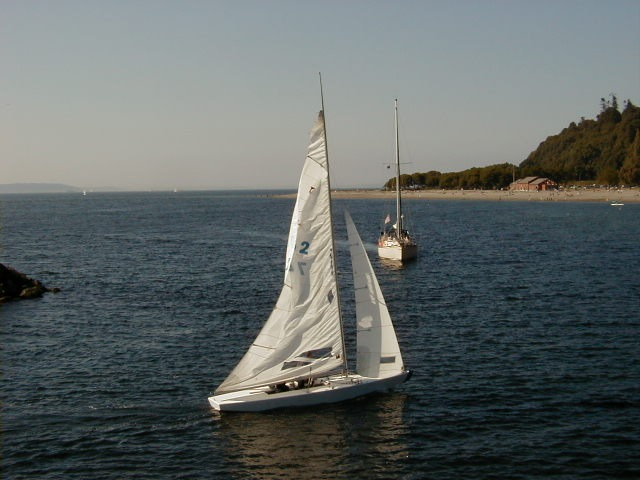
\includegraphics[width=0.9\linewidth]{../input/boat_2.jpg}
	  \caption{1st: boat\_2}
	\end{subfigure}%
	\begin{subfigure}{0.25\textwidth}
        \centering
        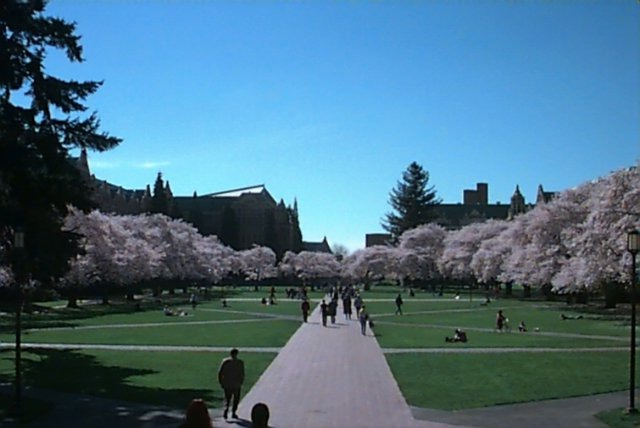
\includegraphics[width=0.9\linewidth]{../input/cherry_3.jpg}
        \caption{2nd: cherry\_3}
    \end{subfigure}%
    \begin{subfigure}{0.25\textwidth}
	  \centering
	  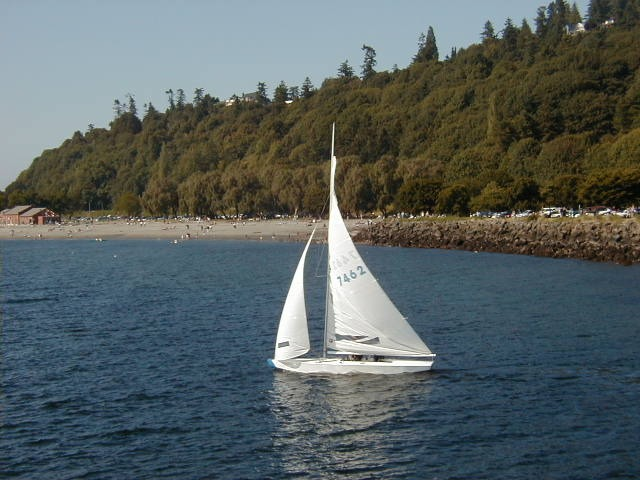
\includegraphics[width=0.9\linewidth]{../input/boat_4.jpg}
	    \caption{3th: boat\_4}
	\end{subfigure}
    \caption{Results for boat\_5}
    \label{fig:results_boat_5}
\end{figure}

\item \textbf{cherry\_3}: cherry\_2, cherry\_1, cherry\_4 (figure \ref{fig:results_cherry_3}).
\begin{figure}[H]
	\centering
	\begin{subfigure}{0.25\textwidth}
	  \centering
	  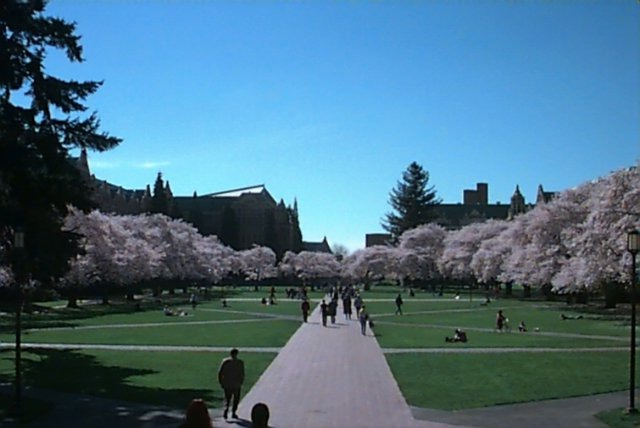
\includegraphics[width=0.9\linewidth]{../input/cherry_3.jpg}
	  \caption{Query: cherry\_3}
	\end{subfigure}%
	\begin{subfigure}{0.25\textwidth}
	  \centering
	  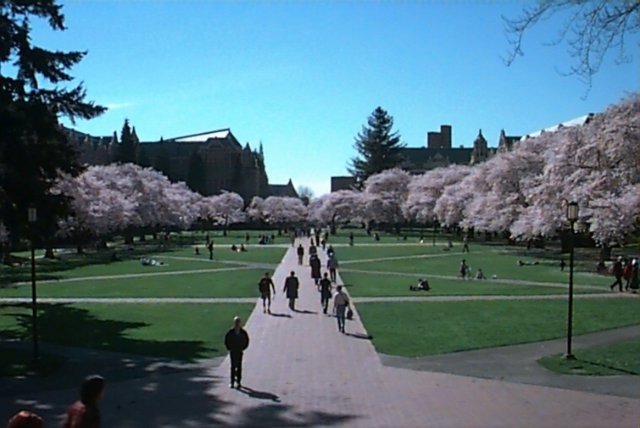
\includegraphics[width=0.9\linewidth]{../input/cherry_2.jpg}
	  \caption{1st: cherry\_2}
	\end{subfigure}%
	\begin{subfigure}{0.25\textwidth}
        \centering
        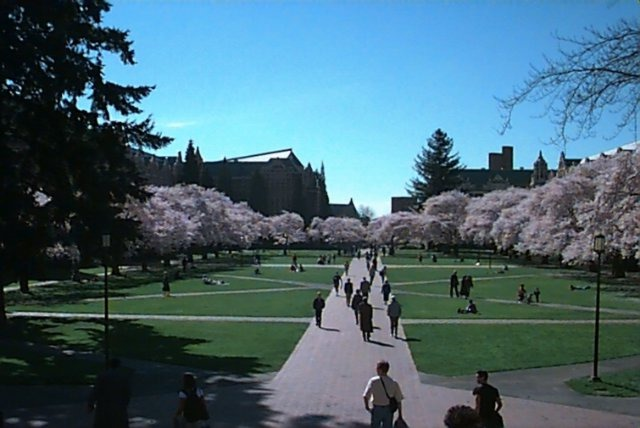
\includegraphics[width=0.9\linewidth]{../input/cherry_1.jpg}
        \caption{2nd: cherry\_1}
    \end{subfigure}%
    \begin{subfigure}{0.25\textwidth}
	  \centering
	  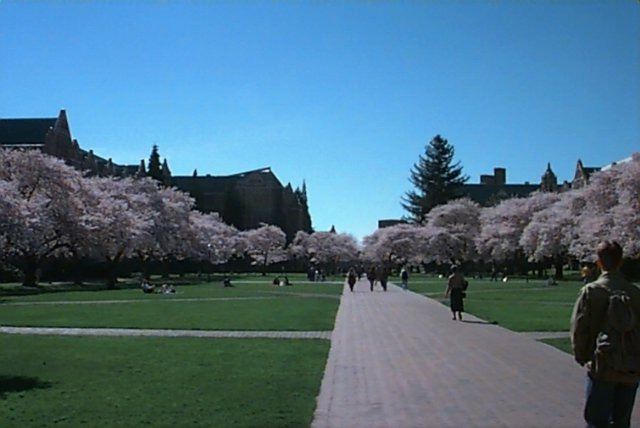
\includegraphics[width=0.9\linewidth]{../input/cherry_4.jpg}
	    \caption{3th: cherry\_4}
	\end{subfigure}
    \caption{Results for cherry\_3}
    \label{fig:results_cherry_3}
\end{figure}


\item \textbf{pond\_2}: pond\_1, pond\_3, boat\_3 (figure \ref{fig:results_pond_2}).

\begin{figure}[H]
	\centering
	\begin{subfigure}{0.25\textwidth}
	  \centering
	  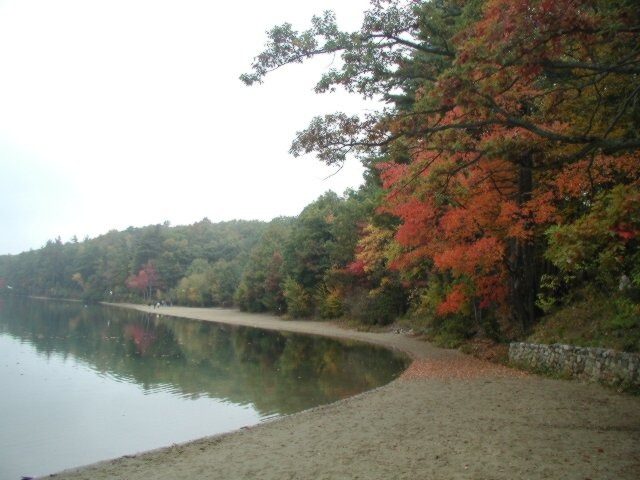
\includegraphics[width=0.9\linewidth]{../input/pond_2.jpg}
	  \caption{Query: pond\_2}
	\end{subfigure}%
	\begin{subfigure}{0.25\textwidth}
	  \centering
	  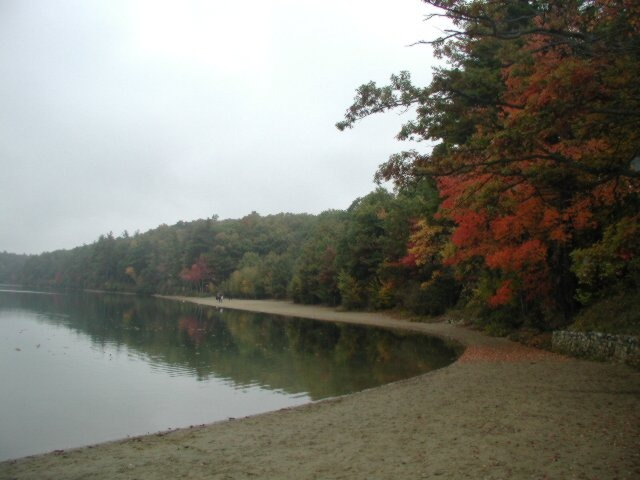
\includegraphics[width=0.9\linewidth]{../input/pond_1.jpg}
	  \caption{1st: pond\_1}
	\end{subfigure}%
	\begin{subfigure}{0.25\textwidth}
        \centering
        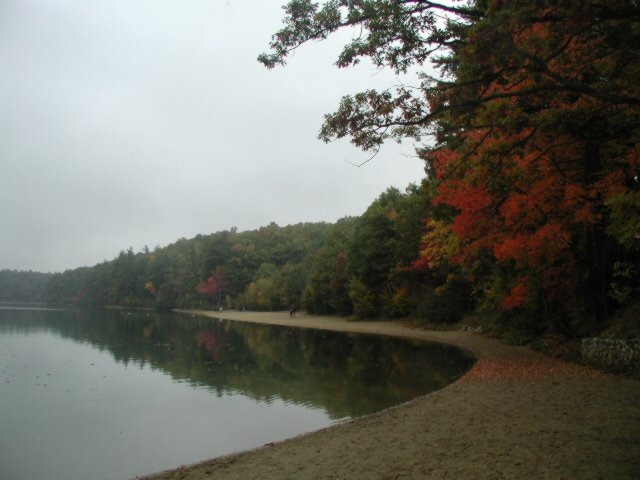
\includegraphics[width=0.9\linewidth]{../input/pond_3.jpg}
        \caption{2nd: bond\_3}
    \end{subfigure}%
    \begin{subfigure}{0.25\textwidth}
	  \centering
	  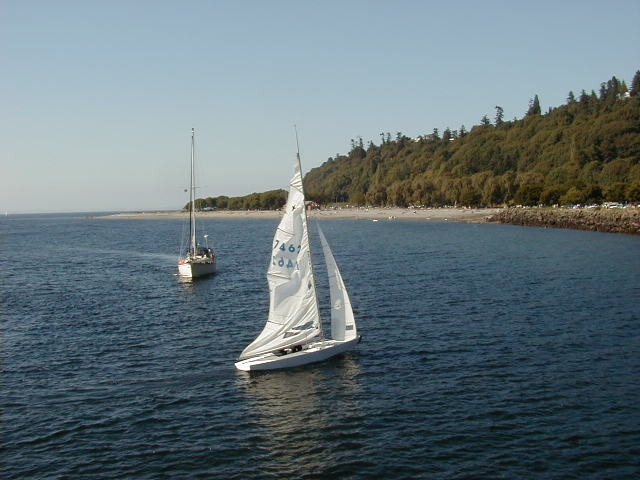
\includegraphics[width=0.9\linewidth]{../input/boat_3.jpg}
	    \caption{3th: boat\_3}
	\end{subfigure}
    \caption{Results for pond\_2}
    \label{fig:results_pond_2}
\end{figure}


\item \textbf{stHelens\_2}: stHelens\_3, stHelens\_5, stHelens\_4 (Figure \ref{fig:results_stHelens_2}).

\begin{figure}[H]
	\centering
	\begin{subfigure}{0.25\textwidth}
	  \centering
	  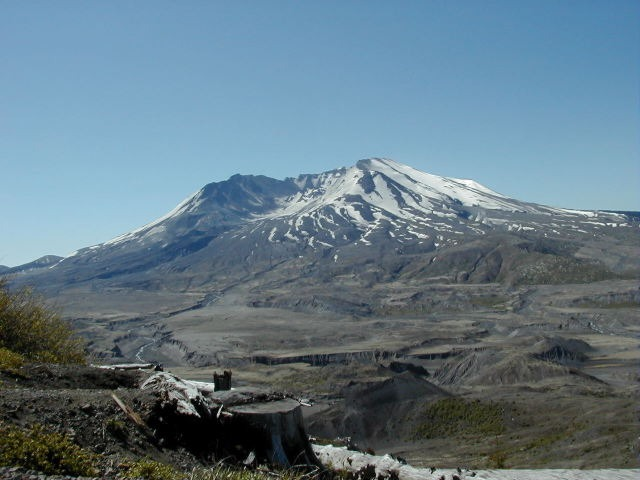
\includegraphics[width=0.9\linewidth]{../input/stHelens_2.jpg}
	  \caption{Query: stHelens\_2}
	\end{subfigure}%
	\begin{subfigure}{0.25\textwidth}
	  \centering
	  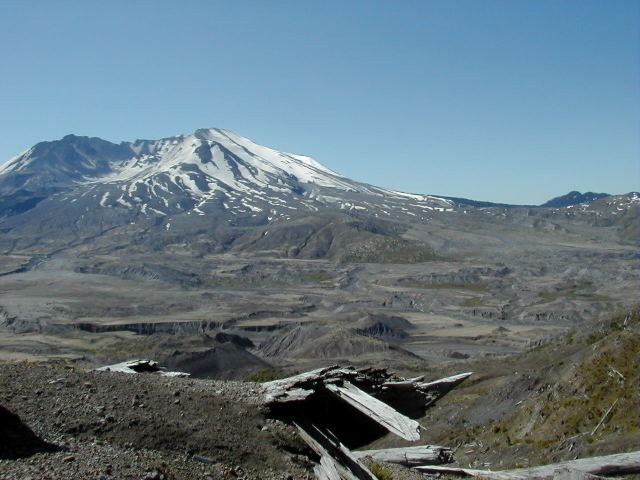
\includegraphics[width=0.9\linewidth]{../input/stHelens_3.jpg}
	  \caption{1st: stHelens\_3}
	\end{subfigure}%
	\begin{subfigure}{0.25\textwidth}
        \centering
        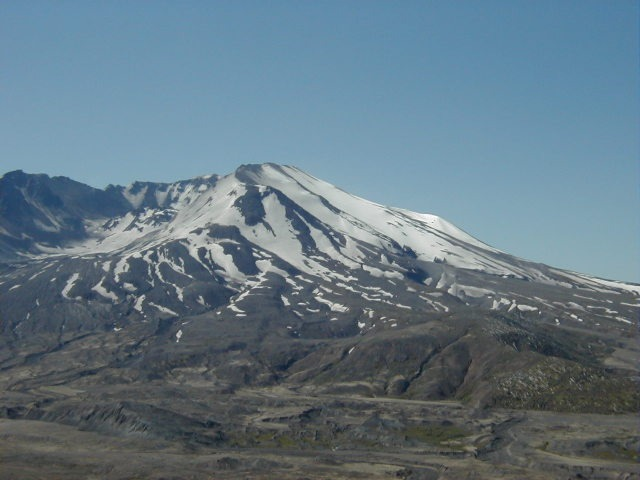
\includegraphics[width=0.9\linewidth]{../input/stHelens_5.jpg}
        \caption{2nd: stHelens\_5}
    \end{subfigure}%
    \begin{subfigure}{0.25\textwidth}
	  \centering
	  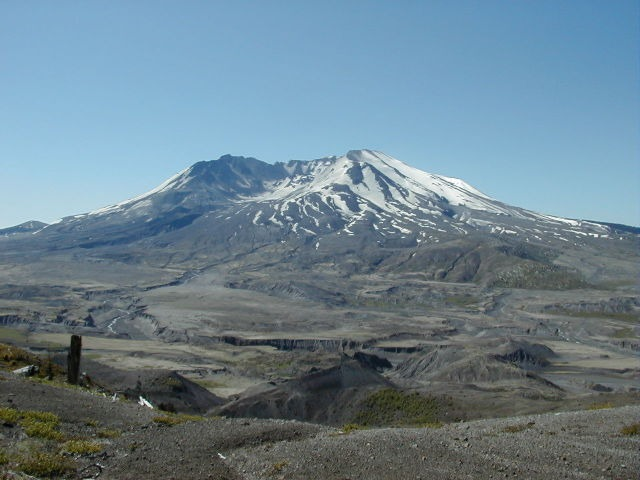
\includegraphics[width=0.9\linewidth]{../input/stHelens_4.jpg}
	    \caption{3th: stHelens\_4}
	\end{subfigure}
    \caption{Results for stHelens\_2}
    \label{fig:results_stHelens_2}
\end{figure}


\item \textbf{sunset1\_2}: sunset1\_1, sunset1\_3, beach\_4 (Figure \ref{fig:results_sunset1_2}). 

\begin{figure}[H]
	\centering
	\begin{subfigure}{0.25\textwidth}
	  \centering
	  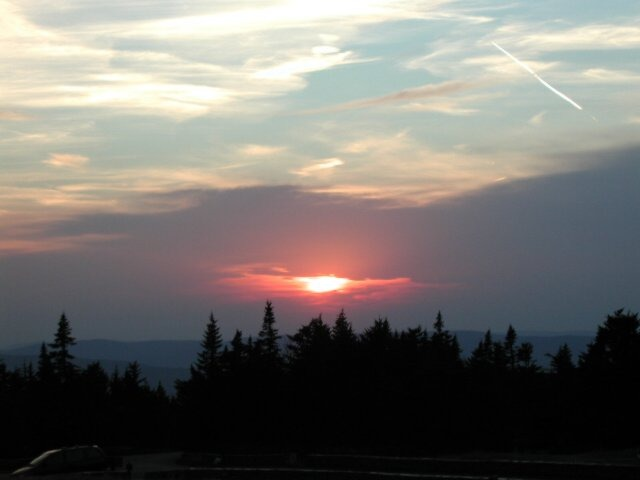
\includegraphics[width=0.9\linewidth]{../input/sunset1_2.jpg}
	  \caption{Query: sunset1\_2}
	\end{subfigure}%
	\begin{subfigure}{0.25\textwidth}
	  \centering
	  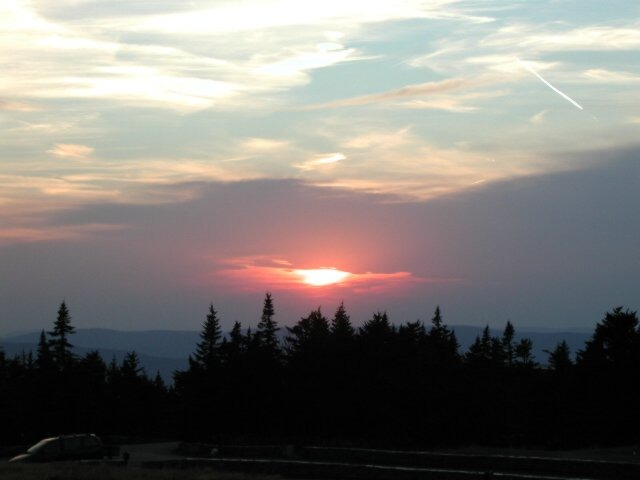
\includegraphics[width=0.9\linewidth]{../input/sunset1_1.jpg}
	  \caption{1st: sunset1\_2}
	\end{subfigure}%
	\begin{subfigure}{0.25\textwidth}
        \centering
        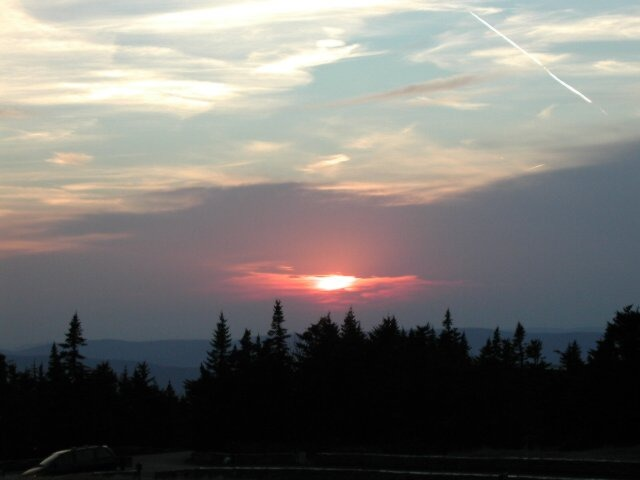
\includegraphics[width=0.9\linewidth]{../input/sunset1_3.jpg}
        \caption{2nd: sunset1\_3}
    \end{subfigure}%
    \begin{subfigure}{0.25\textwidth}
	  \centering
	  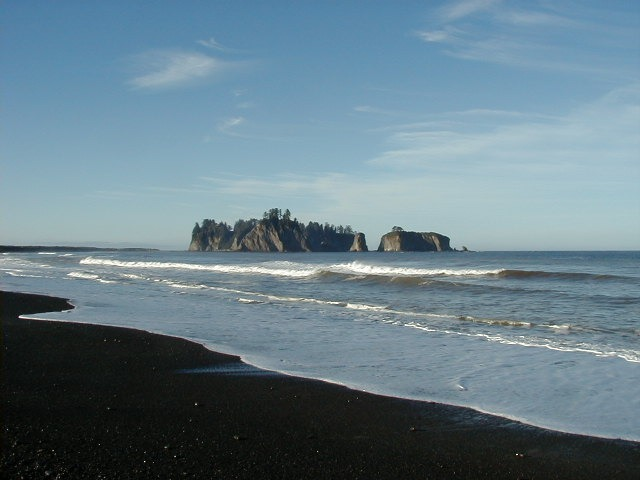
\includegraphics[width=0.9\linewidth]{../input/beach_4.jpg}
	    \caption{3th: beach\_4}
	\end{subfigure}
    \caption{Results for sunset1\_2}
    \label{fig:results_sunset1_2}
\end{figure}

\item \textbf{sunset2\_2}: sunset2\_4, sunset2\_3, beach\_2 (Figure \ref{fig:results_sunset2_2}).

\begin{figure}[H]
	\centering
	\begin{subfigure}{0.25\textwidth}
	  \centering
	  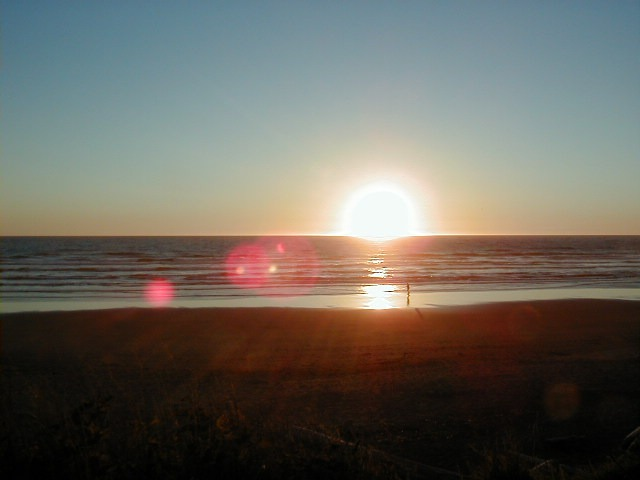
\includegraphics[width=0.9\linewidth]{../input/sunset2_2.jpg}
	  \caption{Query: sunset2\_2}
	\end{subfigure}%
	\begin{subfigure}{0.25\textwidth}
	  \centering
	  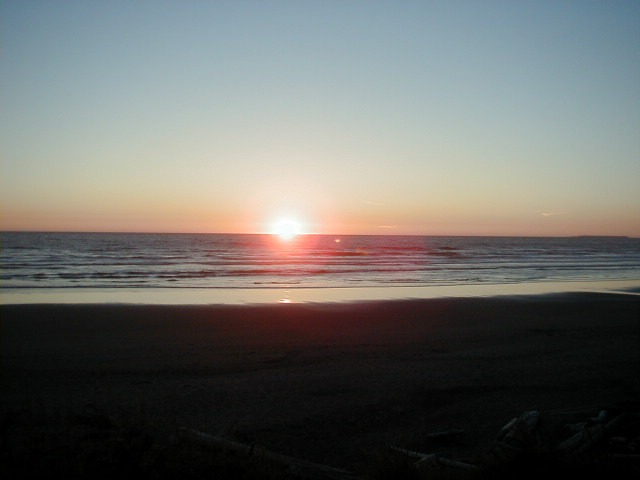
\includegraphics[width=0.9\linewidth]{../input/sunset2_4.jpg}
	  \caption{1st: sunset2\_4}
	\end{subfigure}%
	\begin{subfigure}{0.25\textwidth}
        \centering
        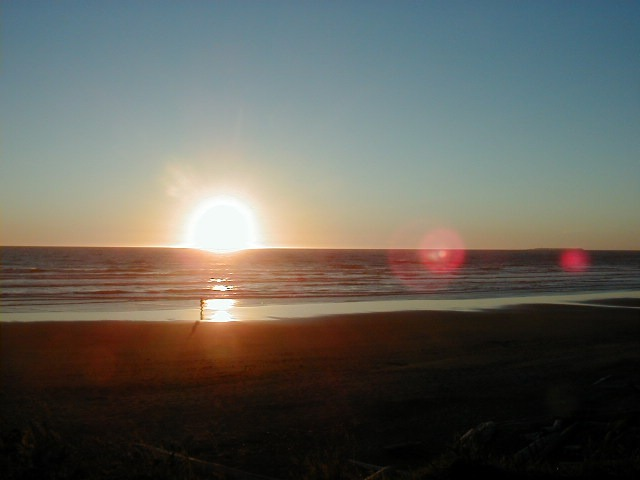
\includegraphics[width=0.9\linewidth]{../input/sunset2_3.jpg}
        \caption{2nd: sunset2\_3}
    \end{subfigure}%
    \begin{subfigure}{0.25\textwidth}
	  \centering
	  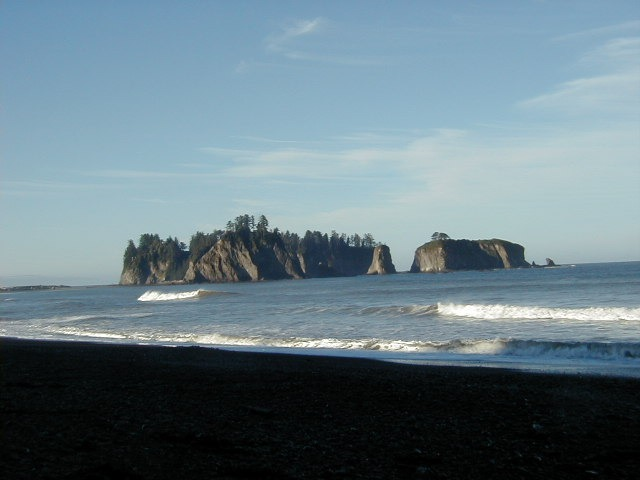
\includegraphics[width=0.9\linewidth]{../input/beach_2.jpg}
	    \caption{3th: beach\_2}
	\end{subfigure}
    \caption{Results for sunset2\_2}
    \label{fig:results_sunset2_2}
\end{figure}

\end{itemize}


\if false
beach_1 ==> [(stHelens_4), (stHelens_5), (stHelens_3)]
beach_2 ==> [(crater_3), (beach_4), (crater_5)]
beach_3 ==> [(beach_4), (beach_2), (beach_1)]
beach_4 ==> [(beach_3), (beach_2), (stHelens_1)]
beach_5 ==> [(stHelens_4), (stHelens_5), (beach_1)]
boat_1 ==> [(stHelens_4), (stHelens_3), (crater_1)]
boat_2 ==> [(boat_3), (boat_5), (cherry_3)]
boat_3 ==> [(boat_2), (boat_5), (boat_4)]
boat_4 ==> [(boat_5), (cherry_3), (boat_3)]
boat_5 ==> [(boat_2), (cherry_3), (boat_4)]
cherry_1 ==> [(cherry_3), (cherry_2), (cherry_5)]
cherry_2 ==> [(cherry_3'), (cherry_1), (cherry_4)]
cherry_3 ==> [(cherry_2), (cherry_1), (cherry_4)]
cherry_4 ==> [(cherry_3), (cherry_2), (cherry_1)]
cherry_5 ==> [(cherry_2), (cherry_3), (cherry_1)]
crater_1 ==> [(stHelens_4), (stHelens_3), (boat_1)]
crater_2 ==> [(crater_5), (crater_4), (crater_3)]
crater_3 ==> [(crater_5), (beach_2'), (crater_4)]
crater_4 ==> [(crater_5), (crater_2), (stHelens_5)]
crater_5 ==> [(crater_4), (crater_2), (stHelens_5)]
pond_1 ==> [(pond_3), (pond_2), (boat_2)]
pond_2 ==> [(pond_1), (pond_3), (boat_3)]
pond_3 ==> [(pond_1), (pond_2), (cherry_3)]
pond_4 ==> [(pond_5), (pond_2), (stHelens_5)]
pond_5 ==> [(pond_4), (cherry_3), (cherry_2)]
stHelens_1 ==> [(cherry_3), (stHelens_5), (cherry_5)]
stHelens_2 ==> [(stHelens_3), (stHelens_5), (stHelens_4)]
stHelens_3 ==> [(stHelens_4), (stHelens_5), (stHelens_2)]
stHelens_4 ==> [(stHelens_3), (stHelens_5), (beach_1)]
stHelens_5 ==> [(stHelens_4), (stHelens_2), (stHelens_3)]
sunset1_1 ==> [(sunset1_3), (sunset1_2), (beach_4)]
sunset1_2 ==> [(sunset1_1), (sunset1_3), (beach_4)]
sunset1_3 ==> [(sunset1_1), (sunset1_2), (beach_4)]
sunset1_4 ==> [(sunset2_1), (beach_3), (beach_4)]
sunset1_5 ==> [(cherry_3), (cherry_2), (beach_1)]
sunset2_1 ==> [(pond_4), (boat_2), (boat_3)]
sunset2_2 ==> [(sunset2_4), (sunset2_3), (beach_2)]
sunset2_3 ==> [(beach_4), (sunset2_2), (beach_2)]
sunset2_4 ==> [(sunset2_2), (sunset2_3), (beach_3)]
sunset2_5 ==> [(crater_3), (beach_2), (cherry_5)]
\fi


